\documentclass[10pt]{article}
\usepackage{icmlko}

\icmlmeta{IP 파운데이션 월드모델}{214}{한철만 있는 열}{공휴일을 2015년까지 채웠더니 축이 살아난 게 아니라 챔피언이 내려앉았다 --- 되찾은 것은 축이 아니라 정직한 수였다}

\begin{document}

\twocolumn[
\icmlheader

\begin{abstract}
노트 213이 ``2023년 이전 공휴일을 채우면 축이 살아난다''를 제일 값싼 다음
칸으로 적었다. 채웠다 --- 영문 위키백과의 음력 명절 표로 여덟 해를 확인해
75개를 \textbf{215개}로 늘렸다(2015-01-01 $\sim$ 2026-12-25). 축이
살아났다: \texttt{cal\_holiday\_gap} 유효 비중이 만화 4.5\%$\to$\textbf{56.9\%}
· 애니 47.7\%$\to$\textbf{100\%} · 웹툰 60.1\%$\to$\textbf{99.0\%} 이고,
노트 213이 잡은 축$\leftrightarrow$시간 $-$0.78$\sim$$-$0.82 는
\textbf{$-$0.21$\sim$$+$0.07} 로 무너진다. \textbf{그런데 판은 안 오른다.}
선형 둘은 정확히 제자리고(F6 $-$0.0005 · $t{=}-0.18$; F21 $+$0.0005 ·
$t{=}0.14$) \textbf{챔피언이 $+$0.4603 에서 $+$0.4396 으로 $-$0.0207
($t{=}-4.74$) 잃는다.} 예측과 반대다. 갈랐다. 설계행렬은 축마다 값과
\emph{관측 지표}를 나란히 싣는데(\texttt{forms.\_design}), 목록이 2023년
부터고 유보가 2025년부터라 그 지표가 \textbf{유보에서 100\% · 학습에서
14$\sim$41\%} 였다. \textbf{유보에서 상수인 열은 순위를 못 매긴다} --- 대신
학습을 배포 시대와 그 이전으로 갈라 주는 스위치로만 쓰인다. 지표를 상수로
묶으면 이전 상태의 챔피언이 $+$0.4603 $\to$ $+$0.4445 로 \textbf{$-$0.0158}
잃고, 채움 상태에서는 $-$0.0034 밖에 안 잃는다. \textbf{그 $+$0.0158 이
노트 213이 남긴 값이었다.} 더 나아간다: 채움 상태에서 \textbf{연휴축을 아예
빼면 챔피언이 오른다}($+$0.4396 $\to$ $+$0.4446). 달력 무리 전체의 트리
우위도 $+$0.0247 에서 \textbf{$+$0.0040} 으로 무너진다. \textbf{달력이
트리에서만 되던 까닭이 여기 있었다} --- 스물다섯 노트를 끈 물음의 답이
``트리가 달력을 잘 쓴다''가 아니라 \textbf{``트리만 시계를 스위치로 쓸 수
있었다''}다. 채움을 채택한다 --- 점수가 아니라 자료가 옳아졌다. 축은 안
뺀다(유의하지 않고 뺄 근거가 점수뿐이다). \textbf{가드 열다섯번째 ``한철''}
을 세웠다: 지표가 유보에서 상수인데 학습에서 0.50 넘게 벌어지면 막는다.
이전 상태를 잡고 채움 상태를 통과시킨다. 라벨을 안 본다.
\end{abstract}
]

\begin{figure*}[t]
\centering
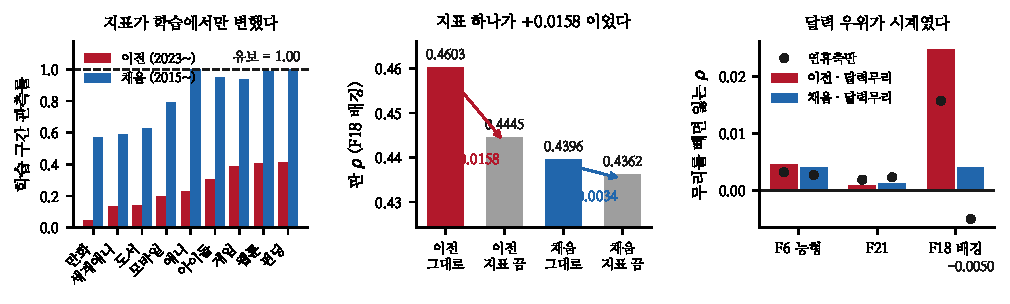
\includegraphics[width=\textwidth]{figs/season.pdf}
\caption{왼쪽 --- 유보는 늘 1.00 이고 학습만 낮았다. 가운데 --- 그 지표
하나가 $+$0.0158. 오른쪽 --- 달력 우위가 무너진다.}
\end{figure*}

\section{채웠고 축은 살아났다}

\begin{table}[t]
\centering\tsize
\caption{\texttt{cal\_holiday\_gap} 유효 비중과 축 $\leftrightarrow$ 시간.}
\begin{tabular}{lrrr}
\toprule
& 이전 & 채움 & 축$\leftrightarrow$시간 \\
\midrule
\textbf{만화} & 4.5\% & \textbf{56.9\%} & $-$.082 \\
세계애니 & 23.7\% & 62.4\% & $+$.008 \\
모바일 & 39.7\% & 83.8\% & $+$.070 \\
\textbf{애니} & 47.7\% & \textbf{100\%} & $-$.022 \\
\textbf{웹툰} & 60.1\% & \textbf{99.0\%} & $+$.073 \\
게임 & 69.9\% & 96.5\% & $+$.005 \\
\bottomrule
\end{tabular}
\end{table}

\claimx{\textbf{여덟 해의 설날 · 부처님오신날 · 추석 양력 날짜를 표로
확인하고}(기억으로 안 적었다) 대체 · 임시공휴일을 붙여 75개를 215개로
늘렸다.}{노트 213이 잡은 축 $\leftrightarrow$ 시간 $-$0.78$\sim$$-$0.82 가
\textbf{$-$0.21$\sim$$+$0.07} 로 무너진다 --- \textbf{시계가 빠졌다.} 그런데
축 $\leftrightarrow$ 라벨도 $+$0.005$\sim$$+$0.10 이다.}

\section{그런데 챔피언이 내려앉는다}

\begin{table}[t]
\centering\tsize
\caption{판 $\rho$. 짝 붓스트랩 500 회.}
\begin{tabular}{lrrrr}
\toprule
& 이전 & 채움 & 차 & $t$ \\
\midrule
F6 능형 & .4293 & .4288 & $-$.0005 & $-$0.18 \\
F21 & .4391 & .4395 & $+$.0005 & $+$0.14 \\
\textbf{F18 배깅} & \textbf{.4603} & \textbf{.4396} & \textbf{$-$.0207} & \textbf{$-$4.74} \\
\bottomrule
\end{tabular}
\end{table}

\claimx{\textbf{자료를 옳게 고쳤는데 챔피언만 $-$0.0207 잃는다.} 선형 둘은
소수 넷째 자리까지 제자리다 --- \textbf{트리만 잃는 것이 있었다.}}{노트 133
대로 첫 수치를 그냥 안 쓴다. \textbf{트리가 무엇을 잃었나.}}

\section{유보에서 상수인 열}

\begin{table}[t]
\centering\tsize
\caption{\texttt{cal\_holiday\_gap} 관측 지표.}
\begin{tabular}{lrrr}
\toprule
& 유보 & 이전 학습 & 채움 학습 \\
\midrule
\textbf{도서} & 1.00 & \textbf{0.14} & 0.62 \\
\textbf{만화} & 1.00 & \textbf{0.04} & 0.57 \\
모바일 & 1.00 & 0.19 & 0.79 \\
\textbf{애니} & 1.00 & \textbf{0.23} & \textbf{1.00} \\
웹툰 & 1.00 & 0.40 & 0.99 \\
펀딩 & 1.00 & 0.41 & 1.00 \\
\bottomrule
\end{tabular}
\end{table}

\claimx{\textbf{설계행렬은 축마다 값과 관측 지표를 나란히 싣는다}
(\texttt{forms.\_design} 의 \texttt{ok.astype(float)}). 목록이 2023년부터고
유보가 2025년부터라 그 지표가 \textbf{유보에서 늘 1 이고 학습에서만
0/1 을 오갔다.}}{\textbf{유보에서 상수인 열은 유보 순위를 못 매긴다.} 대신
학습을 \emph{배포 시대와 그 이전}으로 갈라 주는 스위치로 쓰인다 --- 분할이
시간으로 정의되므로 \textbf{그것은 분할 변수 자체다.}}

\begin{table}[t]
\centering\tsize
\caption{지표를 상수로 묶으면(값은 남긴다). F18 배깅.}
\begin{tabular}{lrrr}
\toprule
& 그대로 & 지표 끔 & 차 \\
\midrule
\textbf{이전} & \textbf{.4603} & .4445 & \textbf{$-$.0158} \\
채움 & .4396 & .4362 & $-$.0034 \\
\bottomrule
\end{tabular}
\end{table}

\claimx{\textbf{그 지표 하나가 $+$0.0158 이었다} --- 노트 213이 얻은 것의
대부분이다. 채움 상태에서는 $-$0.0034 로 준다.}{도메인별로 애니 $+$0.0386 ·
웹툰 $+$0.0184 · 펀딩 $+$0.0170 · 게임 $+$0.0124 다. \textbf{학습 관측률이
낮은 도메인일수록 크다.}}

\section{달력 우위가 시계였다}

\begin{table}[t]
\centering\tsize
\caption{빼면 잃는 $\rho$ (F18 배깅).}
\begin{tabular}{lrr}
\toprule
& 이전 & 채움 \\
\midrule
\textbf{연휴축만} & \textbf{$+$.0157} & \textbf{$-$.0050} \\
\textbf{달력 무리} & \textbf{$+$.0247} & \textbf{$+$.0040} \\
\bottomrule
\end{tabular}
\end{table}

\claimx{\textbf{채움 상태에서는 연휴축을 빼면 챔피언이 오른다}
($+$0.4396 $\to$ $+$0.4446). 달력 무리 전체의 트리 우위도 $+$0.0247 에서
$+$0.0040 으로 무너진다.}{\textbf{``달력이 왜 트리에서만 되는가''는 스물다섯
노트를 끈 물음이고 설명 넷이 실패했다.} 답은 ``트리가 달력을 잘 쓴다''가
아니라 \textbf{``트리만 시계를 스위치로 쓸 수 있었다''}다 --- 능형은 상수
열에 계수를 못 준다.}

\claimx{\textbf{그래도 축은 안 뺀다.} $t{=}1.73$ 으로 유의하지 않고, 뺄
근거가 점수뿐이다 --- 그건 엿보기다.}{\textbf{채움은 점수로 정한 것이
아니다.} 2019년 레코드의 ``다음 연휴까지''는 정의된 양이고, 목록이 없다고
결측으로 두면 \emph{배포 시대 깃발}을 만들어 낸다. 노트 210의 규칙 그대로
점수가 아니라 측정의 유효성으로 정한다.}

\section{가드 한철}

\claimx{\textbf{열다섯번째 가드를 세웠다} --- 지표가 유보에서 상수인데
학습 관측률이 0.50 넘게 벌어지면 막는다. \textbf{라벨을 안 본다} ---
날짜와 결측 무늬만 본다.}{이전 상태에서 일곱 열을 잡고 채움 상태를
통과시킨다. \textbf{노트 213이 ``넷째 층을 가드로''라고 적은 것이
이것이다} --- 자질이 분할 변수를 담는 경우.}

\begin{table}[t]
\centering\tsize
\caption{남은 것.}
\begin{tabular}{ll}
\toprule
\textbf{2015 이전} & 만화 43\% · 세계애니 38\%가 아직 목록 밖 \\
\textbf{노트 186} & 달력 $+$0.140 을 채움 상태에서 다시 잴 것 \\
스위치 & 다른 무리도 학습 전용 열을 갖고 있나 \\
\bottomrule
\end{tabular}
\end{table}

둘째 줄이 제일 크다. 노트 186이 ``달력 무리가 트리 우위의 제일 큰 재료''
라고 $+$0.140 을 쟀고 그 수가 이후 여덟 노트의 전제였다. \textbf{이 노트가
같은 무리를 채움 상태에서 재니 $+$0.0040 이다.} 두 수는 잰 방식이 달라
직접 견줄 수 없지만, \textbf{$+$0.140 이 어느 만큼 시계였는지 같은 틀에서
다시 재야 한다.} 그것이 참이면 트리를 챔피언으로 앉힌 근거 자체가 흔들리고,
\textbf{선형 둘과의 격차 0.021 이 거의 전부 이 한 줄에서 왔을 수 있다.}

\end{document}
